% !TEX root = recommending-interesting-writing.tex
\section{Evaluation}
\label{sec:experiments}

We study the performance of \acrlong{rfs} on a dataset that we collect to assess whether \gls{rfs}, in addition to providing interpretable recommendations to help editors make decisions about articles.

\paragraph{Data collection}

\paragraph{Experimental setup: RankFromSets}

\paragraph{Experimental setup: BERT}

for rankfromsets we searched over 6 embedding sizes [10,25,50, 100, 500, 1000] and 5 batch sizes [500, 1000, 2000, 5000, 10000]. We tried two optimizers, RMS and SGD, both with a momentum of 0.9 and learning rates of [1e-2, 1e-3, 1e-4, 1e-5] for RMS, while learning rates for SGD varied based on batch size and average token count
Breakdown of Data: Train -      Total: 100797            Positive: 18598                 Negative: 82199
Test -      Total: 272448          Positive: 4049                  Negative: 268399
Evaluation -      Total: 272447            Positive: 4039                  Negative: 268348
Both models used the same randomly selected 50k articles from the evaluation set for validation, and the entire test set was used at the end to generate predictions on new data.

\begin{figure}[!tb]
  \centering
  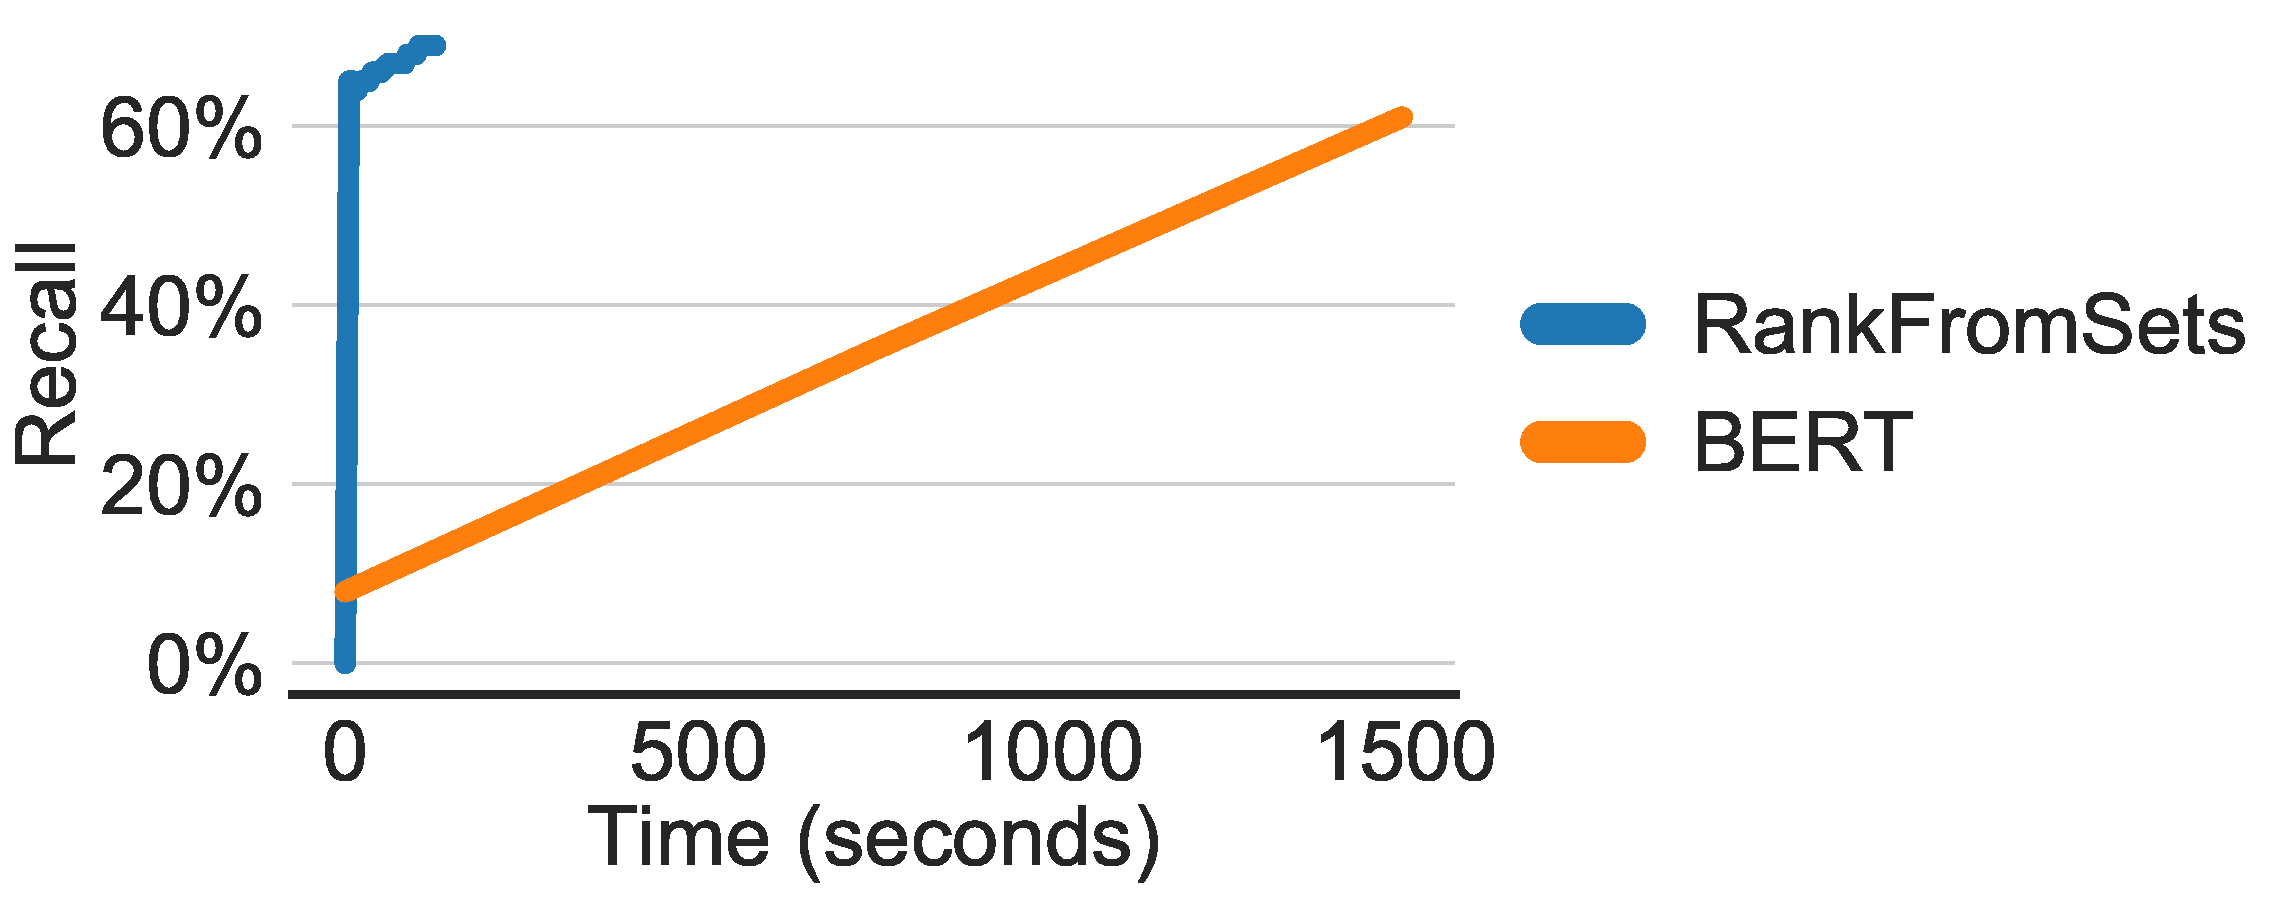
\includegraphics[width=0.95\linewidth]{fig/training-recall}
  \caption{\acrlong{rfs} outperforms models based on word embeddings
    permutation-marginalized recurrent neural networks (denoted by LSTM) on meal
    recommendation. The recommendation models are trained on data from a food
    tracking app as described in \Cref{sec:experiments_meals} and are evaluated
    using the sampled recall metric, \Cref{eq:sampled-recall}. The inner
    product, neural network, and residual regression functions for \acrlong{rfs}
    are in \Cref{eqn:rankfromsets,eqn:neural-network,eqn:residual}.}
  \label{fig:training-recall}
\end{figure}
% !TEX root = ../recommending-interesting-writing.tex
\begin{table}[tb]
\centering
\begin{tabular}{lSS}
\toprule
Recommendation Model & \multicolumn{1}{c}{Recall @ 1000 (\%)}
\\
\midrule
\acrlong{rfs} &  \bfseries 53.1\\
\acrshort{bert} & 46.6 \\
\bottomrule
\end{tabular}
% BERT 466/1000
% rankfromsets 531/1000
% \vspace{1ex}
\caption{\gls{rfs} outperforms \acrshort{bert} in an offline evaluation, on a task of predicting which articles editors at The Browser would feature based on words in the articles.}
\label{tab:recall}
\end{table}

\paragraph{Evaluation.} Qualitatively, editors at The Browser preferred the recommendations of our pipeline over their current workflow of a reading list sorted in terms of recency and use the system in production.